\subsection{Символьное исполнение (symbolic execution)}
\label{symbolic_exec}

\subsubsection{Обмен значений используя исключающее ИЛИ}

Есть хорошо известный (но контринтуитивный) алгоритм для обмена двух значений в двух переменных используя операцию
исключающего ИЛИ, без использования дополнительного регистра/ячейки памяти.

\begin{lstlisting}
X=X^Y
Y=Y^X
X=X^Y
\end{lstlisting}

Как он работает?
Было бы лучше сконструировать выражение на каждом шаге исполнения.

\lstinputlisting{symbolic/1_XOR/xor_swap.py}

Это работает, потому что Питон это \ac{PL} с динамической типизацией, так что ф-ции не важно, над чем работать,
над числами, или над объектами класса Expr().

И вот результат:

\begin{lstlisting}
new_X ((X^Y)^(Y^(X^Y)))
new_Y (Y^(X^Y))
\end{lstlisting}

Можете убрать двойные переменные в уме (т.е., применение исключающего ИЛИ к переменной дважды в итоге ничего не дает).
С new\_X мы можем выбросить два X-а и два Y-а, и остается один Y.
С new\_Y мы можем выбросить два Y-а, и останется один X.

\subsubsection{Смена порядка байт (endianness)}

Что делает этот код?

\begin{lstlisting}
mov     eax, ecx
mov     edx, ecx
shl     edx, 16
and     eax, 0000ff00H
or      eax, edx
mov     edx, ecx
and     edx, 00ff0000H
shr     ecx, 16
or      edx, ecx
shl     eax, 8
shr     edx, 8
or      eax, edx
\end{lstlisting}

На самом деле, многие реверс инженеры играют в игру в наперстки, много, запоминая что где лежит, в каждый момент времени.

\begin{figure}[H]
\centering
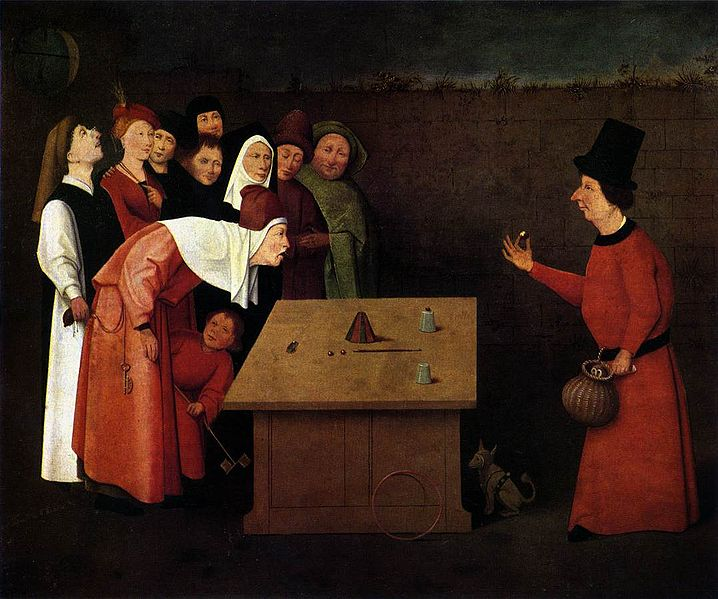
\includegraphics[scale=2.5]{symbolic/2_assembly/718px-Conjurer_Bosch.jpg}
\caption{Иероним Босх -- Фокусник}
\end{figure}

И снова, мы можем сделать эквивалентную ф-цию, которая может брать и переменные с числами и объекты Expr().
Мы также расширяем класс Expr() чтобы он поддерживал многие арифметические и булевы операции.
Также, методы Expr() будут брать на вход и объекты Expr() и целочисленные значения.

\lstinputlisting{symbolic/2_assembly/1.py}

Запускаю:

\begin{lstlisting}
((((initial_ECX&65280)|(initial_ECX<<16))<<8)|(((initial_ECX&16711680)|(initial_ECX>>16))>>8))
\end{lstlisting}

Теперь понятнее, хотя и немного напоминает LISP, с первого взгляда.
На самом деле эта ф-ция меняет порядок байт (endianness) в 32-битном слове.

Кстати, мой игрушечный декомпилятор тоже может это делать, но он оперирует \ac{AST} вместо обычных строк:
\ref{toy_decompiler}.

\subsubsection{Быстрое преобразование Фурье}

Я нашел одну из самых маленьких реализаций FFT на \href{https://www.reddit.com/r/Python/comments/1la4jp/understanding_the_fft_algorithm_with_python/}{реддите}:

\lstinputlisting{symbolic/3_FFT/FFT.py}

Просто интересно, какое значение имеет каждый элемент на выходе?

\lstinputlisting{symbolic/3_FFT/FFT_symb.py}

Ф-ция FFT() оставлена почти без изменений, единственное что я добавил, это то что комплексное значение в начале конвертируется
в строку, и затем конструируется объект Expr().

\lstinputlisting{symbolic/3_FFT/res1.txt}

Мы видим подвыражения вида $x^0$ и $x^1$.
Мы можем их сократить, т.к., $x^0=1$ и $x^1=x$.
Также, мы можем сократить подвыражения вроде $x \cdot 1$ до $x$.

\begin{lstlisting}
    def __mul__(self, other):
        op1=self.s
        op2=self.convert_to_Expr_if_int(other).s

        if op1=="1":
            return Expr(op2)
        if op2=="1":
            return Expr(op1)

        return Expr("(" + op1 + "*" + op2 + ")")

    def __pow__(self, other):
        op2=self.convert_to_Expr_if_int(other).s
        if op2=="0":
            return Expr("1")
        if op2=="1":
            return Expr(self.s)

        return Expr("(" + self.s + "**" + op2 + ")")
\end{lstlisting}

\lstinputlisting{symbolic/3_FFT/res2.txt}

\subsubsection{Циклический избыточный код (\ac{CRC})}

Мне всегда было интересно, какой входной бит влияет на какой бит конечного значения CRC32.

Из теории \ac{CRC} (хорошее и короткое введение:
\url{http://web.archive.org/web/20161220015646/http://www.hackersdelight.org/crc.pdf}
) мы знаем что \ac{CRC} это регистр сдвига с отводами.

Мы будем следить за каждым битом а не байтом или словом, что в свою очередь очень неэффективно, но лучше служит нашим целям.

\lstinputlisting{symbolic/4_CRC/1.py}

Вот выражения для каждого бита CRC32 для 1-байтного буфера:

\lstinputlisting{symbolic/4_CRC/1byte.txt}

Для б\'{о}льших буферов, выражения увеличиваются экспоненциально.
Это 0-й бит конечного состояния для 4-байтного буфера:

\begin{lstlisting}
state 0=((((((((((((((in_0_0^1)^(in_0_1^1))^(in_0_2^1))^(in_0_4^1))^(in_0_5^1))^(in_0_7^(1^(in_0_1^1))))^
(in_1_0^(1^(in_0_2^1))))^(in_1_2^(((1^(in_0_0^1))^(in_0_1^1))^(in_0_4^1))))^(in_1_3^(((1^(in_0_1^1))^
(in_0_2^1))^(in_0_5^1))))^(in_1_4^(((1^(in_0_2^1))^(in_0_3^1))^(in_0_6^(1^(in_0_0^1))))))^(in_2_0^((((1^
(in_0_0^1))^(in_0_6^(1^(in_0_0^1))))^(in_0_7^(1^(in_0_1^1))))^(in_1_2^(((1^(in_0_0^1))^(in_0_1^1))^(in_0_4^
1))))))^(in_2_6^(((((((1^(in_0_0^1))^(in_0_1^1))^(in_0_2^1))^(in_0_6^(1^(in_0_0^1))))^(in_1_4^(((1^(in_0_2^1))^
(in_0_3^1))^(in_0_6^(1^(in_0_0^1))))))^(in_1_5^(((1^(in_0_3^1))^(in_0_4^1))^(in_0_7^(1^(in_0_1^1))))))^
(in_2_0^((((1^(in_0_0^1))^(in_0_6^(1^(in_0_0^1))))^(in_0_7^(1^(in_0_1^1))))^(in_1_2^(((1^(in_0_0^1))^(in_0_1^1))^
(in_0_4^1))))))))^(in_2_7^(((((((1^(in_0_1^1))^(in_0_2^1))^(in_0_3^1))^(in_0_7^(1^(in_0_1^1))))^(in_1_5^(((1^
(in_0_3^1))^(in_0_4^1))^(in_0_7^(1^(in_0_1^1))))))^(in_1_6^(((1^(in_0_4^1))^(in_0_5^1))^(in_1_0^(1^(in_0_2^
1))))))^(in_2_1^((((1^(in_0_1^1))^(in_0_7^(1^(in_0_1^1))))^(in_1_0^(1^(in_0_2^1))))^(in_1_3^(((1^(in_0_1^1))^
(in_0_2^1))^(in_0_5^1))))))))^(in_3_2^(((((((((1^(in_0_1^1))^(in_0_2^1))^(in_0_4^1))^(in_0_5^1))^(in_0_6^(1^
(in_0_0^1))))^(in_1_2^(((1^(in_0_0^1))^(in_0_1^1))^(in_0_4^1))))^(in_2_0^((((1^(in_0_0^1))^(in_0_6^(1^(in_0_0^
1))))^(in_0_7^(1^(in_0_1^1))))^(in_1_2^(((1^(in_0_0^1))^(in_0_1^1))^(in_0_4^1))))))^(in_2_1^((((1^(in_0_1^1))^
(in_0_7^(1^(in_0_1^1))))^(in_1_0^(1^(in_0_2^1))))^(in_1_3^(((1^(in_0_1^1))^(in_0_2^1))^(in_0_5^1))))))^(in_2_4^
(((((1^(in_0_0^1))^(in_0_4^1))^(in_1_2^(((1^(in_0_0^1))^(in_0_1^1))^(in_0_4^1))))^(in_1_3^(((1^(in_0_1^1))^
(in_0_2^1))^(in_0_5^1))))^(in_1_6^(((1^(in_0_4^1))^(in_0_5^1))^(in_1_0^(1^(in_0_2^1))))))))))
\end{lstlisting}

Выражение для 0-го бита конечного состояния 8-байтного буфера имеет длину
$\approx 350KiB$, что, конечно, можно существенно сократить (потому что выражение это дерево из операций исключающего ИЛИ),
но вы можете ощутить его вес.

Теперь мы можем как-нибудь обработать эти выражения, чтобы получить меньшую картину того, что на что влияет.
Скажем так, если мы находим подстроку ``in\_2\_3'' в выражении, это означает что 3-й бит 2-го байта входа влияет на 
это выражение.
И дажее более того, т.к. это дерево из операций исключающего ИЛИ (т.е., выражение состоящее только из этих операций),
если входная переменная встречается дважды, она \textit{аннигилируется}, т.к. $x \oplus x=0$.
Более того: если переменная встречается четное количество раз (2, 4, 8, итд), она аннигилируется,
но остается, если она встречается нечетное кол-во раз (1, 3, 5, итд).

\begin{lstlisting}
    for i in range(32):
        #print "state %d=%s" % (i, state[31-i])
        sys.stdout.write ("state %02d: " % i)
        for byte in range(BYTES):
            for bit in range(8):
                s="in_%d_%d" % (byte, bit)
                if str(state[31-i]).count(s) & 1:
                    sys.stdout.write ("*")
                else:
                    sys.stdout.write (" ")
        sys.stdout.write ("\n")
\end{lstlisting}

( \url{https://github.com/dennis714/SAT_SMT_article/blob/master/symbolic/4_CRC/2.py} )

Вот как каждый бит входного 1-байтного буфера влияет на каждый бит конечного состояния CRC32:

\lstinputlisting{symbolic/4_CRC/1byte_tbl.txt}

Это 8*8=64 бита 8-байтного входного буфера:

\lstinputlisting{symbolic/4_CRC/8byte_tbl.txt}

\subsubsection{Линейный конгруэнтный генератор}

Это популярный \ac{PRNG} из \ac{CRT}-библиотеки OpenWatcom: \url{https://github.com/open-watcom/open-watcom-v2/blob/d468b609ba6ca61eeddad80dd2485e3256fc5261/bld/clib/math/c/rand.c}.

Какое выражение он генерирует на каждом шаге?

\lstinputlisting{symbolic/5_LCG/LCG.py}

\lstinputlisting{symbolic/5_LCG/1.txt}

Теперь, если однажды мы получили несколько значений из этого PRNG, например 4583, 16304, 14440, 32315, 28670, 12568...,
можем ли мы восстановить изначальное состояние генератора?
Эта проблема на самом деле это решение системы уравнений:

\begin{lstlisting}
((((initial_seed*1103515245)+12345)>>16)&32767)==4583
((((((initial_seed*1103515245)+12345)*1103515245)+12345)>>16)&32767)==16304
((((((((initial_seed*1103515245)+12345)*1103515245)+12345)*1103515245)+12345)>>16)&32767)==14440
((((((((((initial_seed*1103515245)+12345)*1103515245)+12345)*1103515245)+12345)*1103515245)+12345)>>16)&32767)==32315
\end{lstlisting}

Как выясняется, Z3 может решить эту систему корректно используя только 2 уравнения:

\lstinputlisting{symbolic/5_LCG/Z3_solve.py}

\begin{lstlisting}
[x = 11223344]
\end{lstlisting}

(Хотя, это требует $\approx 20$ секунд на моем древнем нетбуке на Intel Atom.)

\subsubsection{Констрайнт пути (path constraint)}

Как получить день недели из UNIX-даты?

\begin{lstlisting}
#!/usr/bin/env python

input=...
SECS_DAY=24*60*60
dayno = input / SECS_DAY
wday = (dayno + 4) % 7
if wday==5:
    print "Thanks God, it's Friday!"
\end{lstlisting}

Скажем, нам нужно найти способ исполнить блок с вызовом print().
Какой должен быть вход?

В начале построим выражение для переменной $wday$:

\lstinputlisting{symbolic/6_TGIF/TGIF.py}

\begin{lstlisting}
(((input/86400)+4)%7)
\end{lstlisting}

Чтобы исполнить этот блок, мы должны решить это уравнение: $((\frac{input}{86400}+4) \equiv 5 \mod 7$.

Пока что, это простая задача для Z3:

\lstinputlisting{symbolic/6_TGIF/Z3_solve.py}

\begin{lstlisting}
[x = 86438]
\end{lstlisting}

Это действительно корректная UNIX-дата для пятницы:

\begin{lstlisting}
% date --date='@86438'
Fri Jan  2 03:00:38 MSK 1970
\end{lstlisting}

Хотя и дата имеет 1970-й год, но она верна!

Это также называется ``констрайнт пути'' (``path constraint''), т.е., какой констрайнт должен быть удовлетворен,
чтобы исполнить определнный блок?
Некоторые инструменты имеют слово ``path'' в своих названиях, как
``pathgrind'', 
\href{http://babelfish.arc.nasa.gov/trac/jpf/wiki/projects/jpf-symbc}{Symbolic PathFinder}, CodeSurfer Path Inspector, итд.

Как и игра в наперстки, эта задача очень часто встречается на практике.
Вы можете видеть, что что-то опасное может быть исполнено внутри некоторого бейсик-блока и вы пытаетесь понять,
какие входные значения приведут к его исполнению.
Это может быть переполнение буфера, итд.
Такие входные значения иногда называют ``входные значения смерти'' (``inputs of death'').

Многие кракми решаются таким же образом, всё что вам нужно это найти путь в блок, который выводит ``ключ верен''
или что-то в этом роде.

Мы можем расширить наш крохотный пример:

\begin{lstlisting}
input=...
SECS_DAY=24*60*60
dayno = input / SECS_DAY
wday = (dayno + 4) % 7
print wday
if wday==5:
    print "Thanks God, it's Friday!"
else:
    print "Got to wait a little"
\end{lstlisting}

Теперь у нас два блока: для первого мы должны решить это уравнение: $((\frac{input}{86400}+4) \equiv 5 \mod 7$.
Для второго мы должны решить инвертированное уравнение: $((\frac{input}{86400}+4) \not\equiv 5 \mod 7$.
Решая эти уравнения, мы найдем два пути в оба блока.

KLEE (или похожий инструмент) пытается найти путь в каждый [бейсик] блок и производит ``идеальный'' unit-тест.
Так, KLEE может найти путь в блок, который сваливает процесс, или сообщает о корректности введенного ключа/лицензии, итд.
Удивительно, но KLEE точно так же может находить и бэкдоры.

KLEE также называется ``KLEE Symbolic Virtual Machine'' -- этим создатели хотят подчеркнуть, что KLEE это \ac{VM},
которая исполняет код символьно, а не численно (как обычный \ac{CPU}).

Снова расширим наш крохотный пример.
Мы хотим найти пятницу 13-го. Чтобы всё упростить, ограничим себя 1970-м годом.
Найдем все 12 13-х дней 70-го года:

\lstinputlisting{symbolic/6_TGIF/13th.txt}

Скрипт, проверяющий, является ли текущая дата пятницей 13-го:

\begin{lstlisting}
input=...
SECS_DAY=24*60*60
dayno = input / SECS_DAY
wday = (dayno + 4) % 7
print wday
if wday==5:
    print "Thanks God, it's Friday!"
 
    if dayno in [13,44,72,103,133,164,194,225,256,286,317,347]:
        print "Friday 13th"
\end{lstlisting}

Чтобы добиться исполнения второго "print"-а, мы должны удовлетворить два констрайнта:

\lstinputlisting{symbolic/6_TGIF/Z3_solve2.py}

И это тоже легкая задача для Z3:

\begin{lstlisting}
 % python Z3_solve2.py
[dayno = 316, x = 27302400]
 % date --date='@27302400'
Fri Nov 13 03:00:00 MSK 1970
\end{lstlisting}

Это UNIX-дата, для которой оба констрайнта удовлетворены: 13-ое ноября 1970, пятница.

\subsubsection{Деление на ноль}

Если деление на ноль не \textit{обернуто} проверкой, и исключение не было обработано, это может свалить процесс.

Будем вычислять простое выражение $\frac{x}{2y + 4z - 12}$.
Можем добавить предупреждение в метод \TT{\_\_div\_\_}:

\lstinputlisting{symbolic/7_div/1.py}

\dots так что он будет сообщать об опасных состояниях и условиях:

\begin{lstlisting}
warning: division by zero if (((y*2)+(z*4))-12)==0
(x/(((y*2)+(z*4))-12))
\end{lstlisting}

Уравнение легко решить, попробуем на этот раз Wolfram Mathematica:

\begin{lstlisting}
In[]:= FindInstance[{(y*2 + z*4) - 12 == 0}, {y, z}, Integers]
Out[]= {{y -> 0, z -> 3}}
\end{lstlisting}

Эти значения для $y$ и $z$ также можно назвать ``inputs of death''.

% FIXME translation
\subsubsection{Сортировка слиянием (merge sort)}

Как работает сортировка слиянием (merge sort)?
Я скопипастил Питоновский исходник из rosettacode.com, почти без изменений:

\lstinputlisting{symbolic/8_sorting/1.py}

Но здесь есть ф-ция которая сравнивает элементы.
Очевидно, без нее ничего работать не будет.

Так что мы будем хранить и выражения для каждого элемента, и численные значения.
В итоге выведутся оба.
Но когда значения будут сравниваться, будут использоваться только численные части.

Результат:

\lstinputlisting{symbolic/8_sorting/result.txt}

\subsubsection{Расширение класса Expr}

Это наверное бессмысленно, но тем не менее, легко расширить класс Expr для поддержки \ac{AST} вместо обычных строк.
Можно также добавить шаги для сокращения выражения (как я показал в игрушечном декомпиляторе: \ref{toy_decompiler}).
Может быть, кто-то захочет сделать это как упражнение.
Кстати, мой игрушечный декомпилятор может использоваться как простейший symbolic engine --- просто подавайте ему на вход
все инструкции, и он будет следить за состоянием каждого регистра.

\subsubsection{Вывод}

Ради демонстрации, я всё сделал настолько просто, насколько это возможно.
Но реальность всегда намного жестче и неудобнее, так что всё это не нужно воспринимать как серебряную пулю.

Файлы использованные в этой части: \url{https://github.com/dennis714/SAT_SMT_article/tree/master/symbolic}.

